\section*{Ejercicio \#2}
Como paso siguiente procedemos a implementar los algoritmos de ordenamiento a continuación:
\begin{itemize}
    \item \href{https://github.com/syordya/CSUNSA-EDA/tree/master/Practica01/code/BubbleSort}{\textbf{Bubble Sort}}: Complejidad $O(n^2)$.
    \item \href{https://github.com/syordya/CSUNSA-EDA/tree/master/Practica01/code/CountingSort}{\textbf{Counting sort}}: Complejidad $O(n+k)$
    \item \href{https://github.com/syordya/CSUNSA-EDA/tree/master/Practica01/code/HeapSort}{\textbf{Heap sort}} : Complejidad $O(nlogn)$.
    \item \href{https://github.com/syordya/CSUNSA-EDA/tree/master/Practica01/code/InsertionSort}{\textbf{Insertion sort}} : Complejidad $O(n^2)$ \cite{cormen}.
    \item \href{https://github.com/syordya/CSUNSA-EDA/tree/master/Practica01/code/MergeSort}{\textbf{Merge sort}}: Complejidad $O(n log n)$.
    \item \href{https://github.com/syordya/CSUNSA-EDA/tree/master/Practica01/code/QuickSort}{\textbf{Quick sort}}: Complejidad $O(nlogn)$.
    \item \href{https://github.com/syordya/CSUNSA-EDA/tree/master/Practica01/code/SelectionSort}{\textbf{Selection sort}}: Complejidad $O(n^2)$.
\end{itemize}

Para esta tarea usamos los lenguajes \verb!C++!, \verb!Java! y \verb!Python!. Las implementaciones se encuentra en la carpeta \href{https://github.com/syordya/CSUNSA-EDA/tree/master/Practica01/code}{code} del repositorio de la Práctica01.

Para ejecutar los algoritmos en el lenguaje \verb!C++! lo realizamos de la siguiente forma, pasando como entrada, al ejecutable, el archivo \verb!entrada.txt!, el cual contiene los vectores de números aleatorios generados previamente.%Ver figura \ref{fig:ejecucion-cpp}.
\begin{figure}[H]
  \centering
  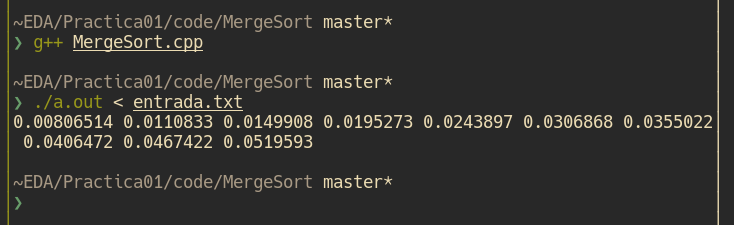
\includegraphics[width=0.8\textwidth]{ejecucion-cpp}
  \label{fig:ejecucion-cpp}
\end{figure}

De la misma forma en \verb!Python!.% Ver figura \ref{fig:ejecucion-python}
\begin{figure}[H]
  \centering
  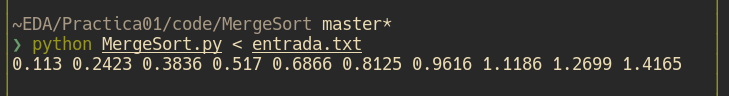
\includegraphics[width=0.8\textwidth]{ejecucion-python}
  \label{fig:ejecucion-python}
\end{figure}

y en \verb!Java!.% Ver figura \ref{fig:ejecucion-java}
\begin{figure}[H]
  \centering
  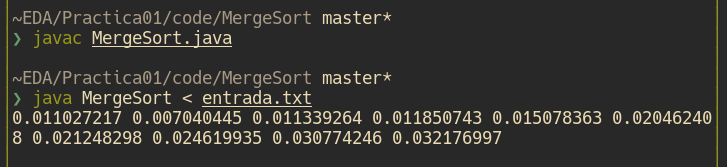
\includegraphics[width=0.8\textwidth]{ejecucion-java}
  \label{fig:ejecucion-java}
\end{figure}

\iffalse
% ---- Para poner dos imágenes (una a lado de otra) ----
Como se muestra en la figuras \ref{fig:act-1_a} y \ref{fig:act-1_b}.
\begin{figure}[H]
\centering
\begin{minipage}{0.45\textwidth}
  \centering
  \includegraphics[width=0.9\textwidth]{act-1_a}
  \caption{Envío de \textit{ICMP ECHO REQUEST} de PC0 a PC1, PC2 y PC3.}
  \label{fig:act-1_a}
\end{minipage}\hfill
\begin{minipage}{0.45\textwidth}
  \centering
  \includegraphics[width=0.9\textwidth]{act-1_b}
  \caption{Respuesta de PC1, PC2 y PC3. Tabla ARP de PC0.}
  \label{fig:act-1_b}
\end{minipage}
\end{figure}
% ---- Para colocar una imagen ----
Como se muestra en la figura \ref{fig:act-3}
\begin{figure}[H]
  \centering
  \includegraphics[width=0.8\textwidth]{act-3}
  \caption{Tabla de subneteo para la red 192.168.100.0.}
  \label{fig:act-3}
\end{figure}
\fi